% style/preamble throws error, hence preamble4tex is kept here
\documentclass[11pt,compress,t,notes=noshow]{beamer}\usepackage[]{graphicx}\usepackage[]{color}

\makeatletter
\def\maxwidth{ %
  \ifdim\Gin@nat@width>\linewidth
    \linewidth
  \else
    \Gin@nat@width
  \fi
}
\makeatother

\definecolor{fgcolor}{rgb}{0.345, 0.345, 0.345}
\newcommand{\hlnum}[1]{\textcolor[rgb]{0.686,0.059,0.569}{#1}}%
\newcommand{\hlstr}[1]{\textcolor[rgb]{0.192,0.494,0.8}{#1}}%
\newcommand{\hlcom}[1]{\textcolor[rgb]{0.678,0.584,0.686}{\textit{#1}}}%
\newcommand{\hlopt}[1]{\textcolor[rgb]{0,0,0}{#1}}%
\newcommand{\hlstd}[1]{\textcolor[rgb]{0.345,0.345,0.345}{#1}}%
\newcommand{\hlkwa}[1]{\textcolor[rgb]{0.161,0.373,0.58}{\textbf{#1}}}%
\newcommand{\hlkwb}[1]{\textcolor[rgb]{0.69,0.353,0.396}{#1}}%
\newcommand{\hlkwc}[1]{\textcolor[rgb]{0.333,0.667,0.333}{#1}}%
\newcommand{\hlkwd}[1]{\textcolor[rgb]{0.737,0.353,0.396}{\textbf{#1}}}%
\let\hlipl\hlkwb

\usepackage{framed}
\makeatletter
\newenvironment{kframe}{%
 \def\at@end@of@kframe{}%
 \ifinner\ifhmode%
  \def\at@end@of@kframe{\end{minipage}}%
  \begin{minipage}{\columnwidth}%
 \fi\fi%
 \def\FrameCommand##1{\hskip\@totalleftmargin \hskip-\fboxsep
 \colorbox{shadecolor}{##1}\hskip-\fboxsep
     \hskip-\linewidth \hskip-\@totalleftmargin \hskip\columnwidth}%
 \MakeFramed {\advance\hsize-\width
   \@totalleftmargin\z@ \linewidth\hsize
   \@setminipage}}%
 {\par\unskip\endMakeFramed%
 \at@end@of@kframe}
\makeatother

\definecolor{shadecolor}{rgb}{.97, .97, .97}
\definecolor{messagecolor}{rgb}{0, 0, 0}
\definecolor{warningcolor}{rgb}{1, 0, 1}
\definecolor{errorcolor}{rgb}{1, 0, 0}
\definecolor{code}{rgb}{0.97, 0.96, 1.0}
\newenvironment{knitrout}{}{} % an empty environment to be redefined in TeX

\usepackage{alltt}
\usepackage[utf8]{inputenc}
\usepackage[ngerman]{babel}
\usepackage{dsfont}
\usepackage{verbatim}
\usepackage{amsmath}
\usepackage{amsfonts}
\usepackage{mathtools}
\usepackage{csquotes}
\usepackage{cmbright}
\usepackage{multirow}
\usepackage{longtable}
\usepackage{enumerate}
\usepackage[absolute,overlay]{textpos}
\usepackage{psfrag}
\usepackage{algorithm}
\usepackage{algpseudocode}
\usepackage{eqnarray}
\usepackage{bytefield}
\usepackage{animate}
\usepackage{tikz}
\usetikzlibrary{shapes,matrix,positioning,chains,arrows,shadows,decorations.pathmorphing,fit,backgrounds}
\usepackage{adjustbox}
\usepackage{colortbl}
\usepackage{tabularx} % for tables (incl. \hline)
\usepackage{arydshln} % Load after array, longtable, colortab and/or colortbl , otherwise problems with \hline in tabular env
\usepackage{etex} %increase registers for \dimenS to more than 256, otherwise we get "No room for a new \dimen"
\usepackage{graphicx}
\usepackage{booktabs} %used in epr lectures
\usepackage{bm} % bold greek letters
\usepackage{hyperref} % url citing
\usepackage{blkarray} % block arrays
\usepackage{listings} % block of code
\usepackage{xcolor} %colored math symbols
\usepackage{pgffor}
\usepackage{verbatimbox}
\usepackage{xcolor}

%some colors
\definecolor{checkgreen}{HTML}{18A126}
\definecolor{errorred}{HTML}{FF0000}
\definecolor{blockbg}{HTML}{F7F7F7}
\definecolor{gray}{HTML}{A0A0A0}

% basic latex stuff
\newcommand{\col}{\par\colorbox{code}{\parbox{\textwidth}{\theverbbox}}\par}
\newcommand{\eg}{e.\,g.\xspace} %for example
\newcommand{\ie}{i.\,e.\xspace} %that is to say...
\newcommand{\pkg}[1]{{\fontseries{b}\selectfont #1}} %fontstyle for R packages
\newcommand{\lz}{\vspace{0.5cm}} %vertical space
\newcommand{\oneliner}[1] % Oneliner for important statements
{\begin{block}{}\begin{center}\begin{Large}#1\end{Large}\end{center}\end{block}}
\def\SpAr{\quad \Rightarrow \quad}

%new environments
\newenvironment{vbframe}  %frame with breaks and verbatim
{
 \begin{frame}[containsverbatim,allowframebreaks]
}
{
\end{frame}
}

\newenvironment{vframe}  %frame with verbatim without breaks (to avoid numbering one slided frames)
{
 \begin{frame}[containsverbatim]
}
{
\end{frame}
}

\newenvironment{blocki}[1]   % itemize block
{
 \begin{block}{#1}\begin{itemize}
}
{
\end{itemize}\end{block}
}

\newenvironment{fragileframe}[2]{  %fragile frame with framebreaks
\begin{frame}[allowframebreaks, fragile, environment = fragileframe]
\frametitle{#1}
#2}
{\end{frame}}

\newcommand{\myframe}[2]{  %short for frame with framebreaks
\begin{frame}[allowframebreaks]
\frametitle{#1}
#2
\end{frame}}

\usepackage{../../style/lmu-lecture}

\let\code=\texttt
\let\proglang=\textsf

\setkeys{Gin}{width=0.9\textwidth}

\usepackage{tikz}
\usetikzlibrary{shapes,arrows,snakes, calc}

% Define block styles
\tikzstyle{decision} = [diamond, draw, text width=6em, text badly centered, node distance=4cm, inner sep=0pt]
\tikzstyle{decision2} = [diamond, draw, fill=customgreen!35, text width=6em, text badly centered, node distance=4cm, inner sep=0pt]

\tikzstyle{block} = [rectangle, draw, text width=14em, text centered, rounded corners, node distance=3cm, minimum height=4em]
\tikzstyle{line} = [draw, -latex']
\tikzstyle{cloud} = [draw, ellipse, node distance=3cm, minimum height=2em]

\title{Introduction to Deep Learning}
\author{Bernd Bischl}
\institute{Department of Statistics -- LMU Munich}
\date{WS 2021/2022}

\setbeamertemplate{frametitle}{\expandafter\uppercase\expandafter\insertframetitle}

\IfFileExists{upquote.sty}{\usepackage{upquote}}{}
\input{../../latex-math/basic-math}
\input{../../latex-math/basic-ml}
\input{../../latex-math/ml-nn}

\newcommand{\titlefigure}{figure/front.png}
\newcommand{\learninggoals}{
  \item CNNs Introduction
}

\title{Deep Learning}
\date{}

\begin{document}

\lecturechapter{CNN: Introduction}
\lecture{I2DL}
%%%%%%%%%%%%%%%%%%%%%%%%%%%%%%%%%%%%%%%%%%%%%%%%%%%%%%%%%%%%%%%%%%

\begin{vbframe}{Convolutional Neural Networks}
\begin{itemize}
\item Convolutional Neural Networks (CNN, or ConvNet) are a powerful family of neural networks that are inspired by biological process in which the connectivity pattern between neurons resembles the organization of the mamel visual cortex.
\end{itemize}
\begin{figure}
\centering
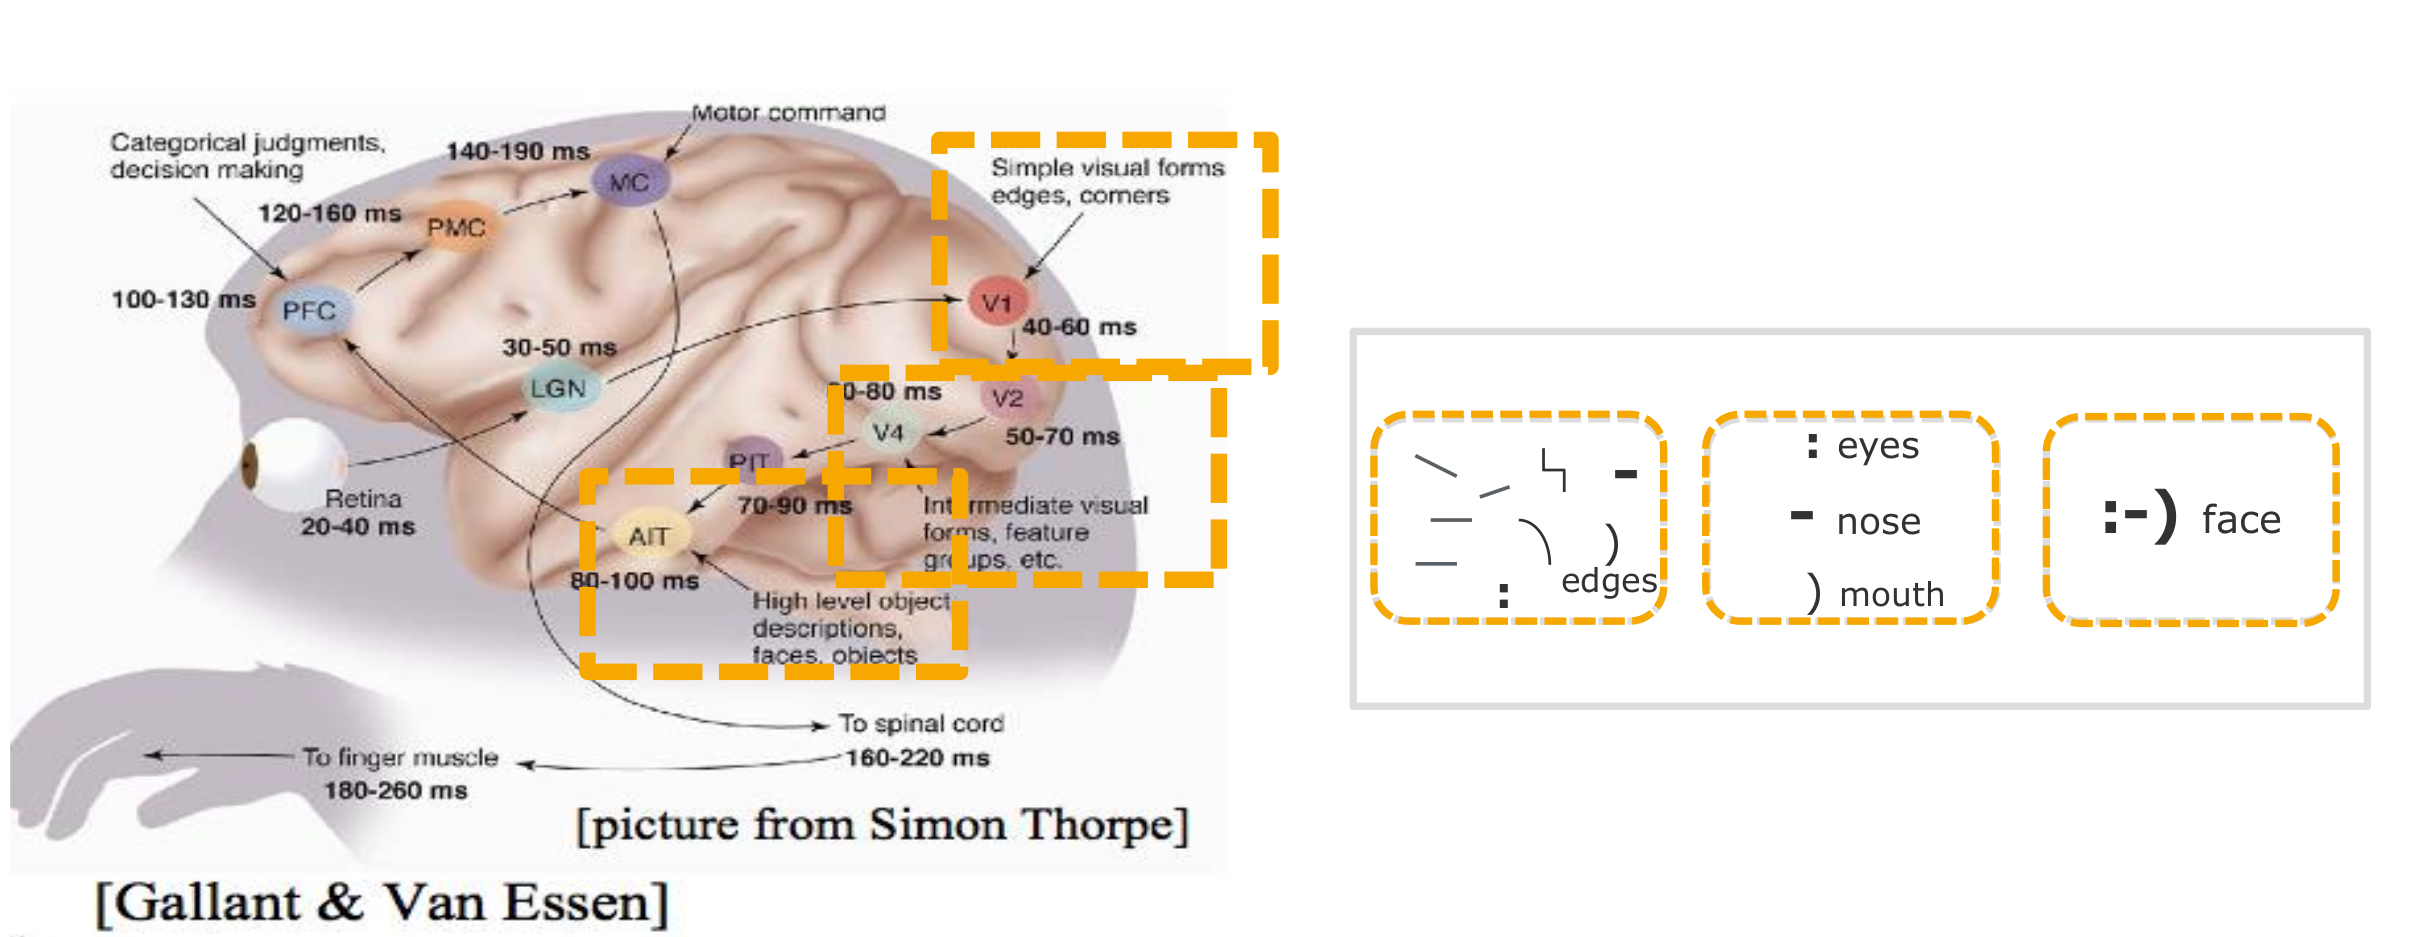
\includegraphics[width=8cm]{figure/cortex.png}
\caption{The ventral (recognition) pathway in the visual cortex has multiple stage: Retina - LGN - V1 - V2 - V4 - PIT - AIT ...., lots of intermediate representations}
\end{figure}
\framebreak
%%%%%%%%%%%%%%%%%%%%%%%%%%%%%%%%%%%%%%%%%%%%%%%%%%%%%%%%%%%%%%%%%%

\begin{itemize}
    \item Since 2012, by the success of CNNs model in ILSVRC compition, they are popular in many fields such as computer vision.
    \item Common applications of CNN-based architectures in computer vision are:
    \begin{itemize}
      \item Image classification.
      \item Object detection /localization.
      \item Semantic segmentation.
    \end{itemize}
    \item Also widely applied in other domains such as natural language processing (NLP), Speech and even time-series data.
\item Basic idea: a CNN automatically extracts visual, or, more generally, spatial features from an input such that it is able to make the optimal prediction based on the extracted features.
\item Therefore, it contains different building blocks and components. 
\end{itemize}
\end{vbframe}

%%%%%%%%%%%%%%%%%%%%%%%%%%%%%%%%%%%%%%%%%%%%%%%%%%%%%%%%%%%%%%%%%%

\begin{vbframe}{CNNs - What for?}
  \begin{figure}
    \centering
    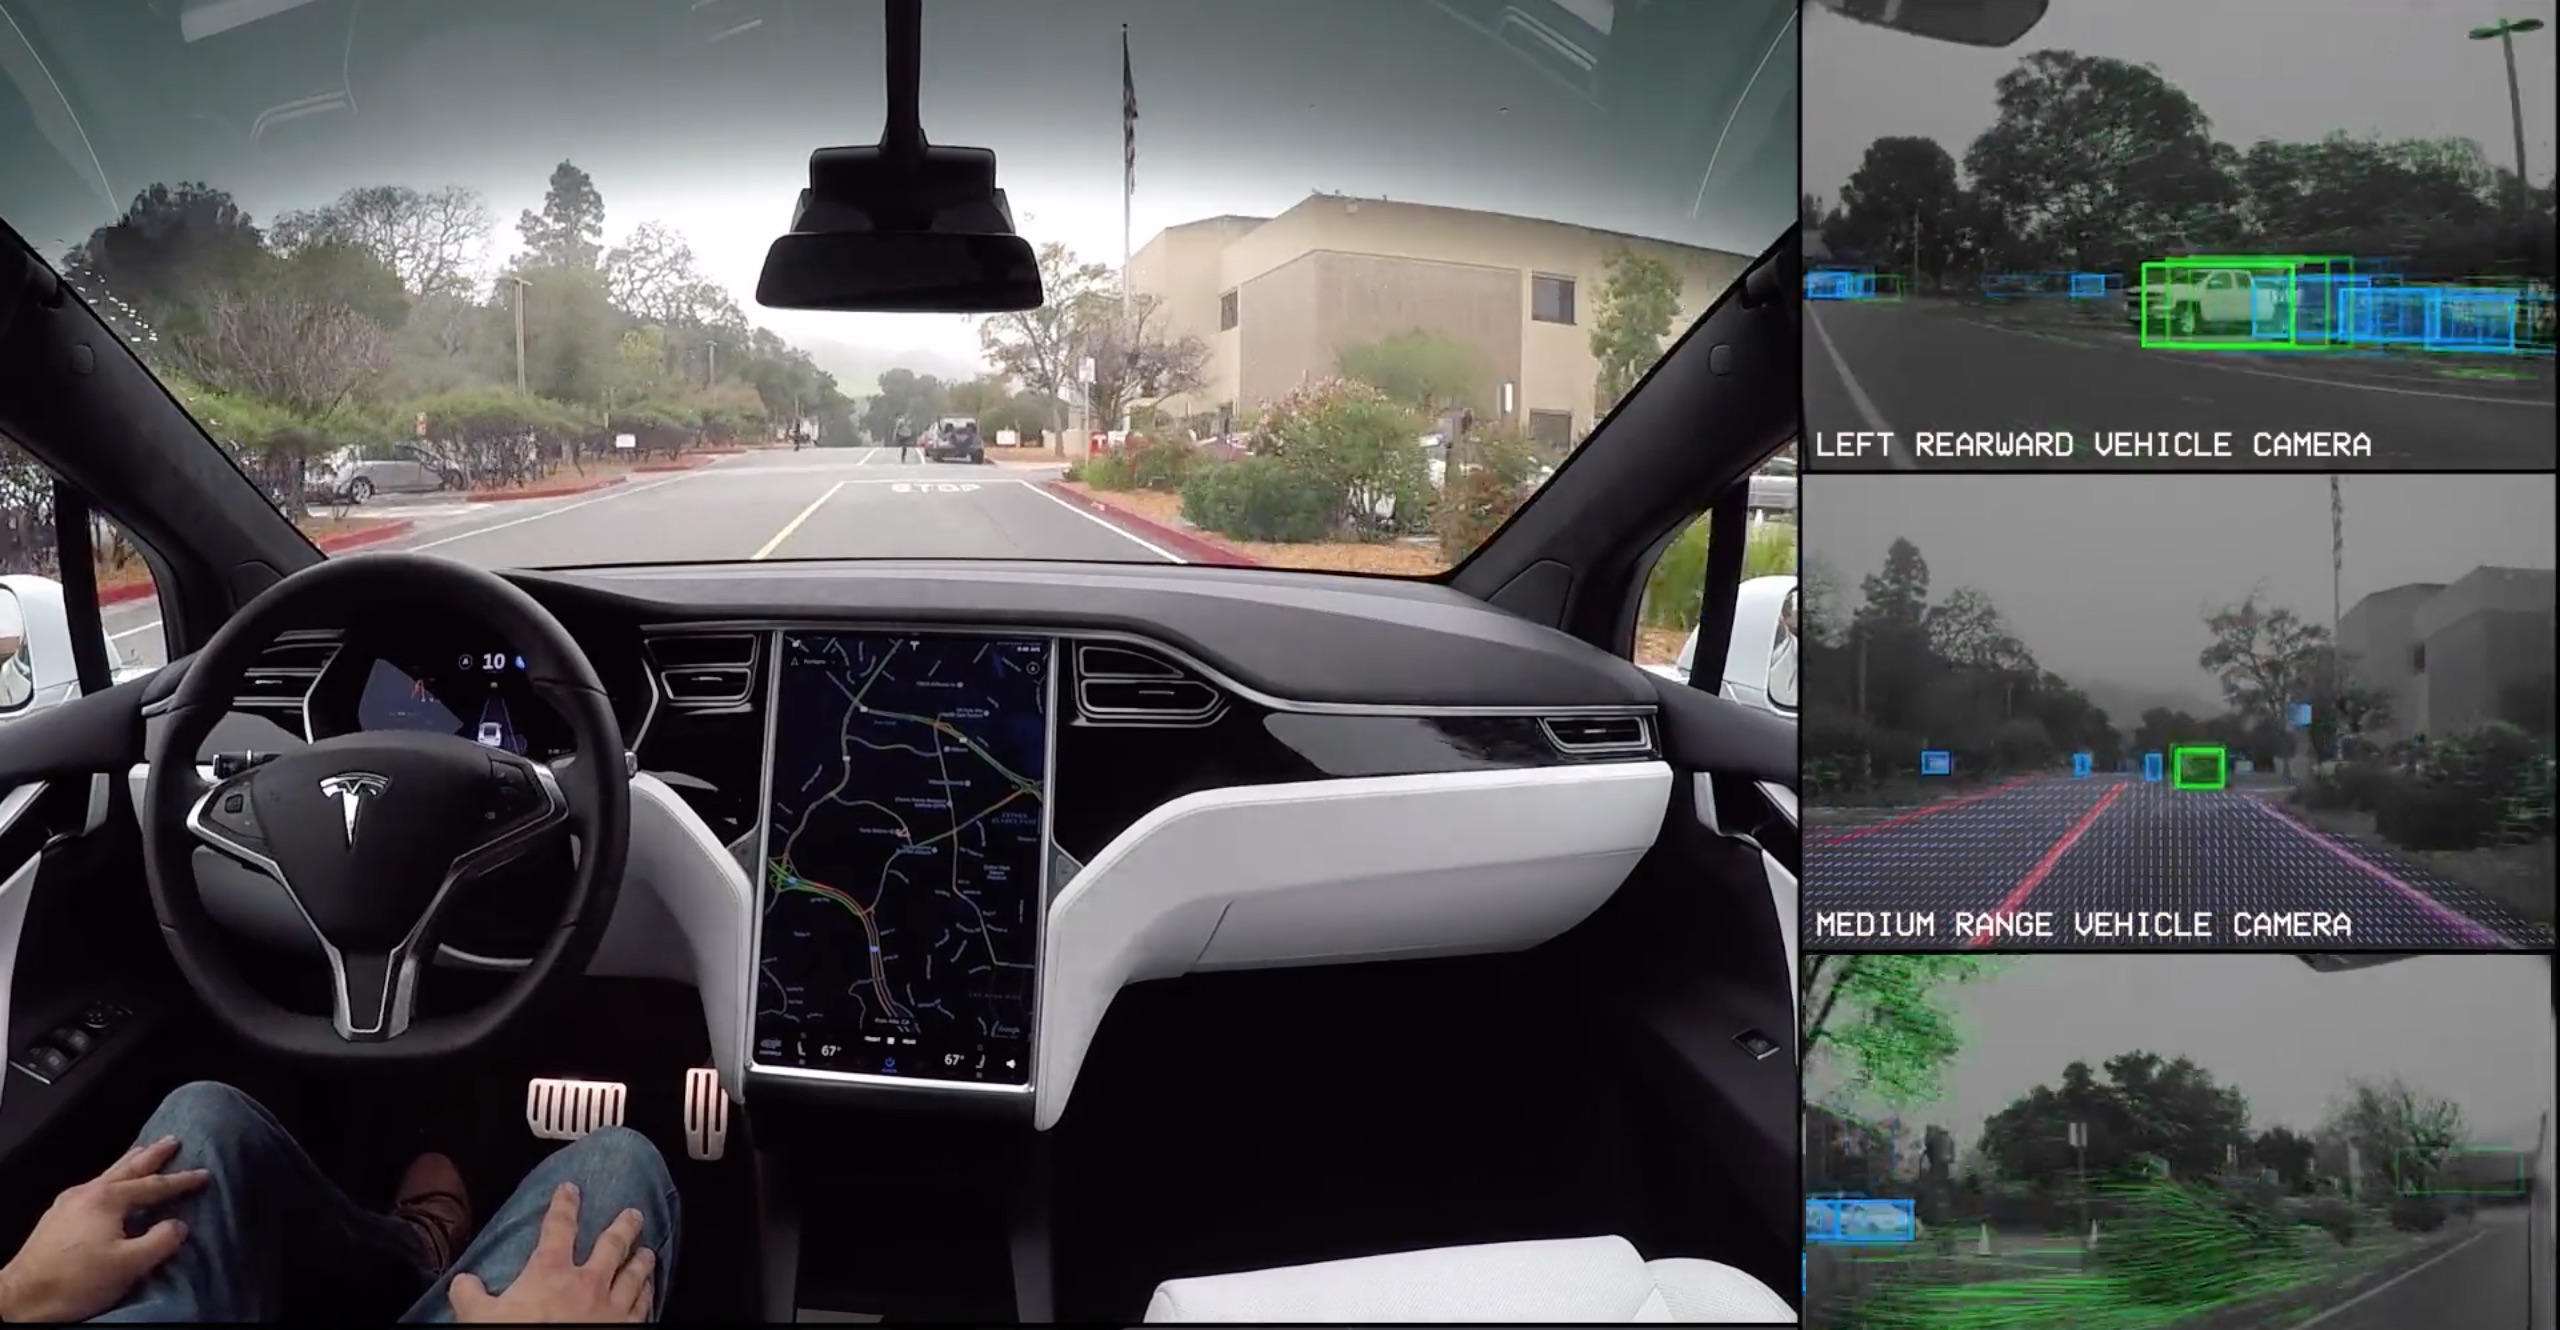
\includegraphics[width=7cm]{figure/tesla_autopilot.jpg}
    \caption{All Tesla cars being produced now have full self-driving hardware and customers can purchase one today (source Tesla website) .Twenty-nine states from fifty states in the U.S. have enacted legislation related to autonomous vehicles. A convolutional neural network is used to map raw pixels from a single front-facing camera directly into steering commands. With minimum training data from humans, the system learns to drive in traffic on local roads with or without lane markings and on highways.}
  \end{figure}
\framebreak
%%%%%%%%%%%%%%%%%%%%%%%%%%%%%%%%%%%%%%%%%%%%%%%%%%%%%%%%%%%%%%%%%%

\begin{figure}
    \centering
    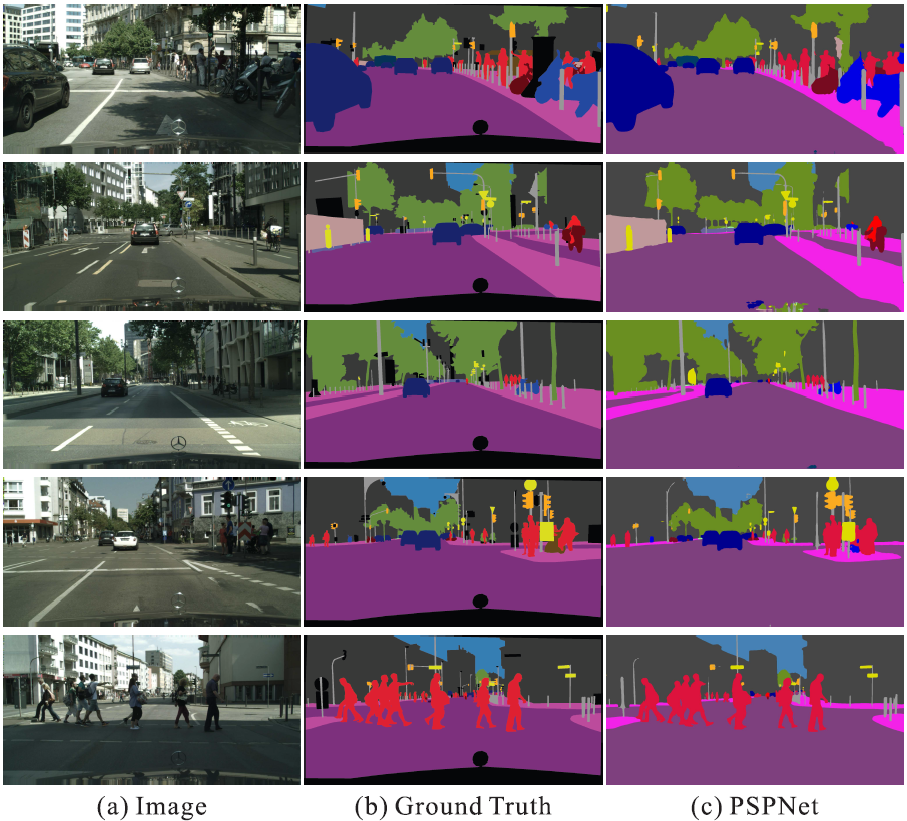
\includegraphics[width=5cm]{figure/cityscapes_visual.png}
    \caption{Given an input image, first CNN is used to get the feature map of the last convolutional layer, then a pyramid parsing module is applied to harvest different sub-region representations, followed by upsampling and concatenation layers to form the final feature representation, which carries both local and global context information. Finally, the representation is fed into a convolution layer to get the final per-pixel prediction. (Source: pyramid scene parsing network,by Zhao et. al, CVPR 2017) }
  \end{figure}
\framebreak
%%%%%%%%%%%%%%%%%%%%%%%%%%%%%%%%%%%%%%%%%%%%%%%%%%%%%%%%%%%%%%%%%%

  \begin{figure}
    \centering
    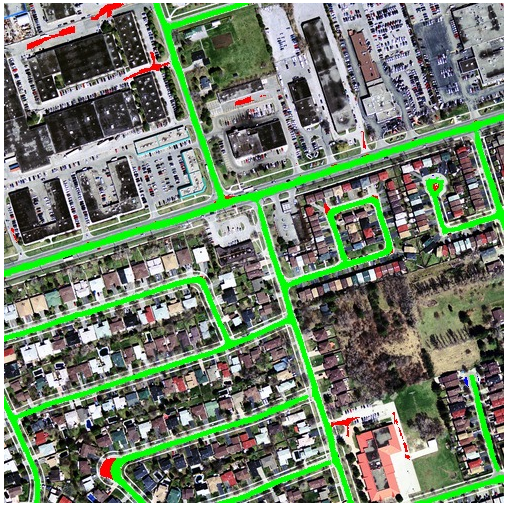
\includegraphics[width=6cm]{figure/road_seg.png}
    \caption{Road segmentation (Mnih Volodymyr (2013)). Aerial images and possibly outdated map pixels are labeled.}
  \end{figure}
\framebreak
%%%%%%%%%%%%%%%%%%%%%%%%%%%%%%%%%%%%%%%%%%%%%%%%%%%%%%%%%%%%%%%%%%

\begin{wrapfigure}{R}{0.5\textwidth}
  \centering
  \scalebox{0.5}{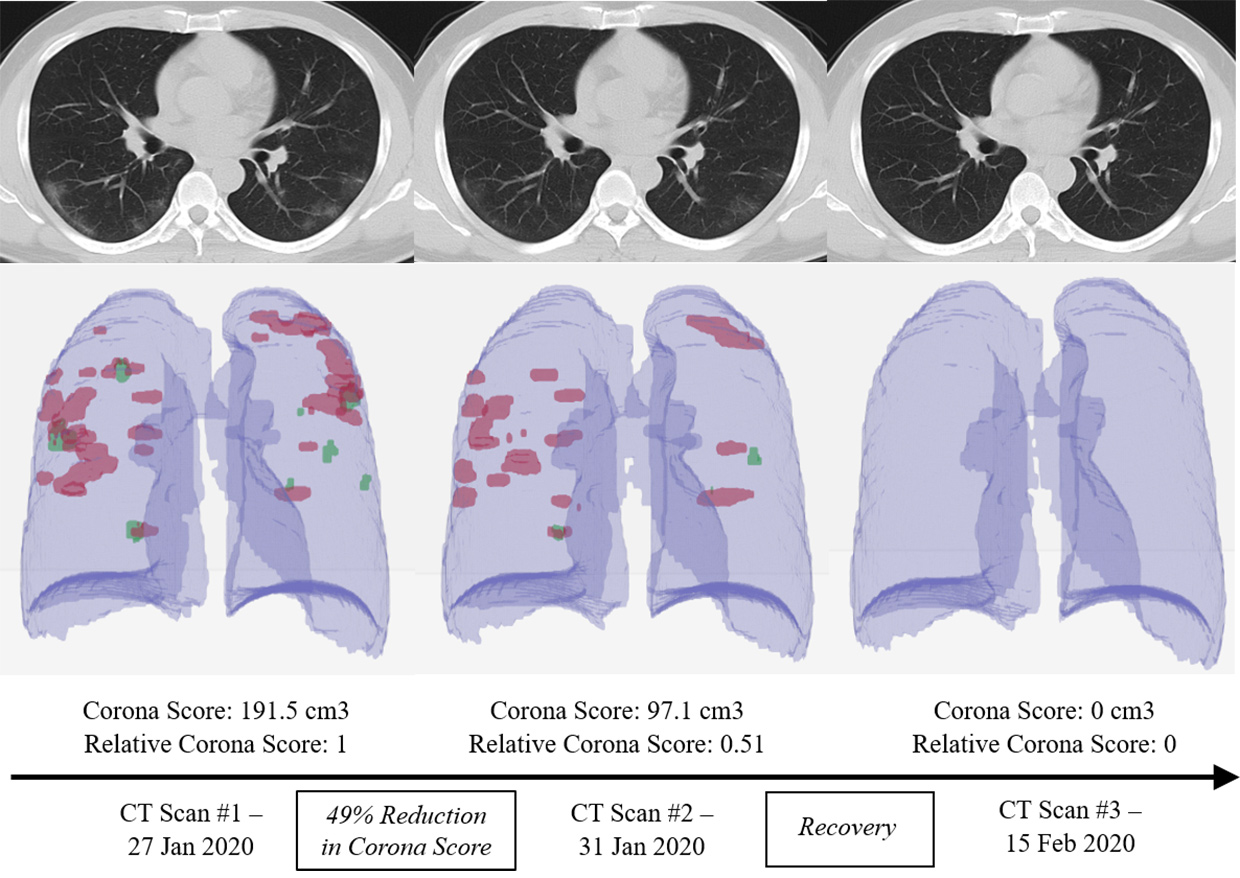
\includegraphics{figure/coronatrack.jpeg}}
\end{wrapfigure}

{CNN for personalized medicine: tracking, diagnosis and localization of Covid-19 patient}
  \begin{itemize}
    \item CNN based model (RADLogists) for personalized Covid-19 detection: three CT scans from a single coronavirus patient diagnosed by RADLogists 
  \end{itemize}
  
   \begin{figure}
    \centering
    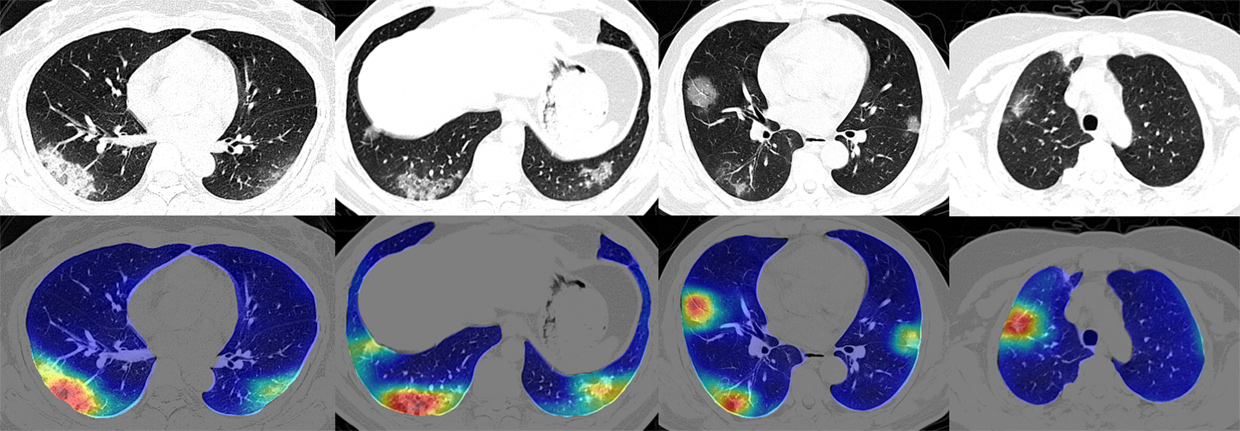
\includegraphics[width=6cm]{figure/hitmap.jpeg}
    \caption{Four COVID-19 lung CT scans (top) with corresponding colored maps showing coronavirus abnormalities (bottom).(source: IEEE Spectrum)}
  \end{figure}
\framebreak
%%%%%%%%%%%%%%%%%%%%%%%%%%%%%%%%%%%%%%%%%%%%%%%%%%%%%%%%%%%%%%%%%%

  \begin{figure}
    \centering
    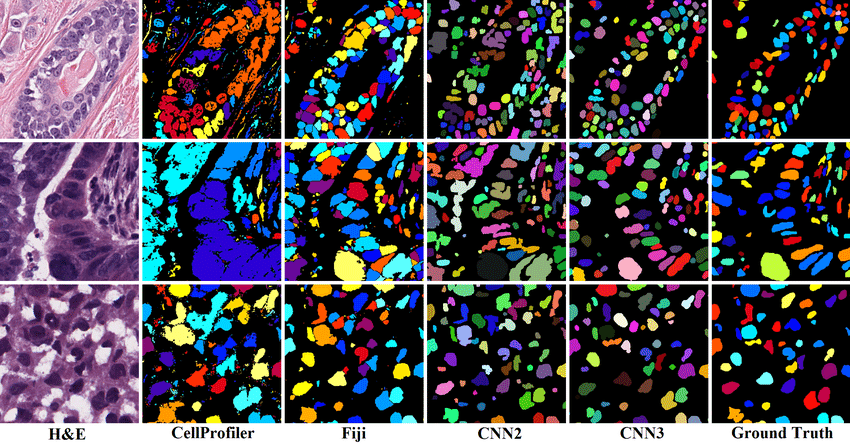
\includegraphics[width=9cm]{figure/instanceseg.png}
    \caption{Nuclear segmentation in digital microscopic tissue images can enable extraction of high-quality features for nuclear morphometrics and other analysis in computational pathology. (source: Kummar et. al. IEEE Transaction Medical Imaging) }
  \end{figure}
\framebreak
%%%%%%%%%%%%%%%%%%%%%%%%%%%%%%%%%%%%%%%%%%%%%%%%%%%%%%%%%%%%%%%%%%

  \begin{figure}
    \centering
    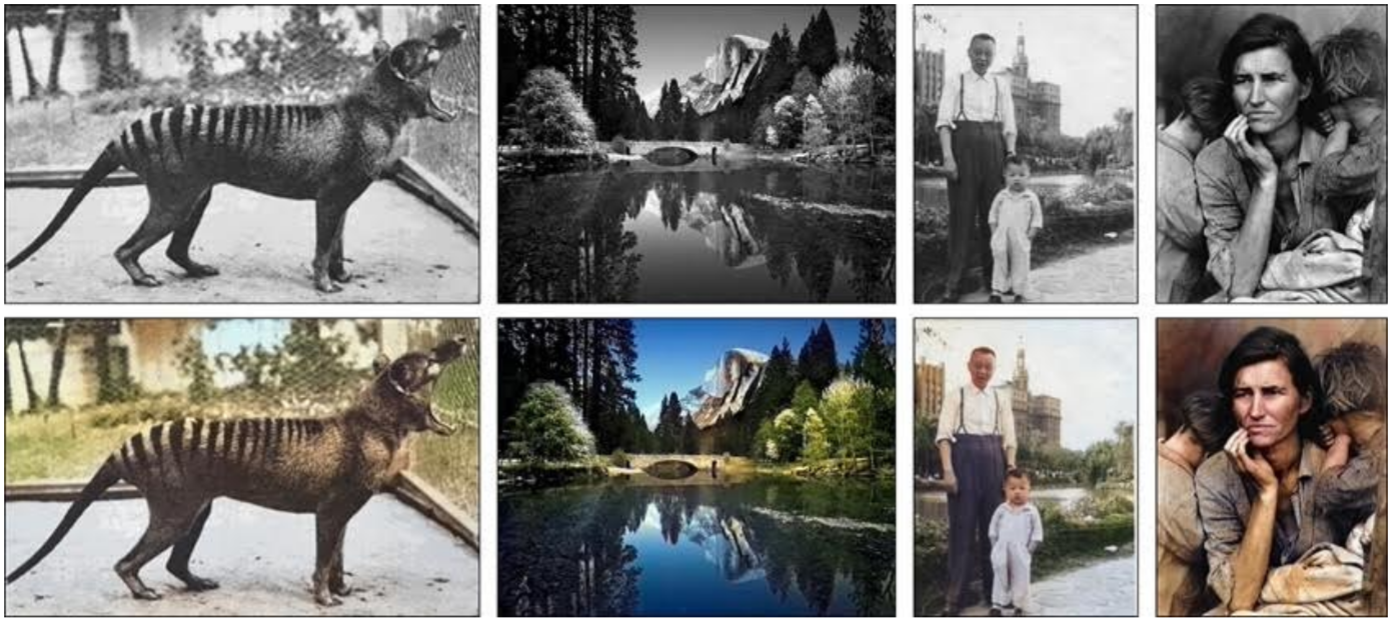
\includegraphics[width=11cm]{figure/colorization.png}
    \caption{Colorful Image Colorization (Zhang et al. (2016)). Given a grayscale photograph as input (top row), this network attacks the problem of hallucinating a plausible color version of the photograph (bottom row, i.e. the prediction of the network). Realizing this task manually consumes many hours of time.}
  \end{figure}
\framebreak

%%%%%%%%%%%%%%%%%%%%%%%%%%%%%%%%%%%%%%%%%%%%%%%%%%%%%%%%%%%%%%%%%%

  \begin{figure}
    \centering
    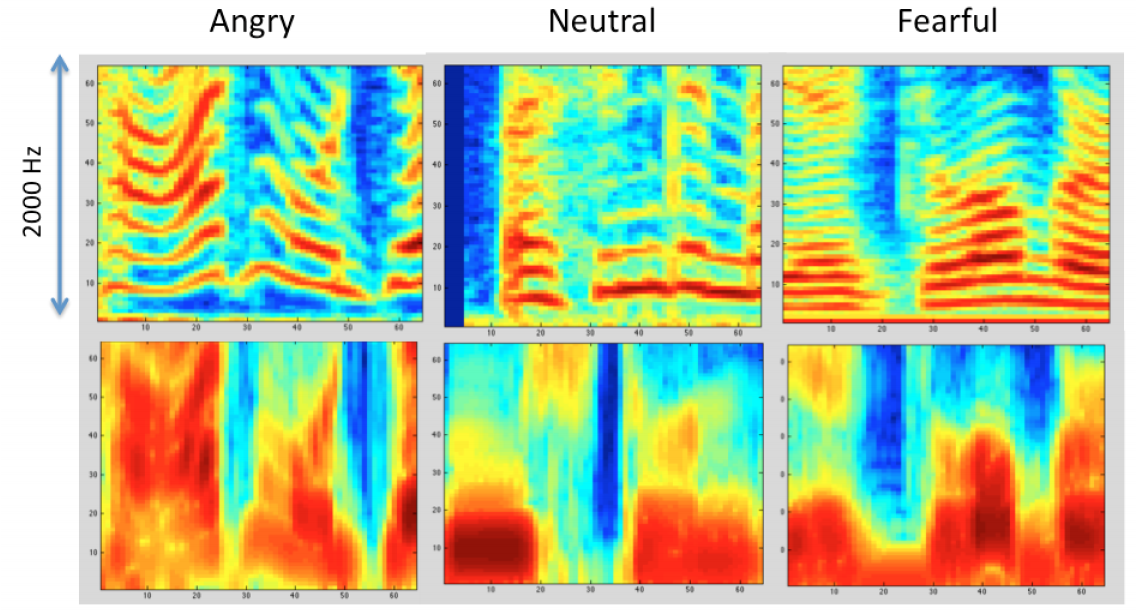
\includegraphics[width=10cm]{figure/speech.png}
    \caption{Speech recognition (Anand \& Verma (2015)). Convolutional neural network to extract features from audio data in order to classify emotions.}
  \end{figure}
\end{vbframe}
%%%%%%%%%%%%%%%%%%%%%%%%%%%%%%%%%%%%%%%%%%%%%%%%%%%%%%%%%%%%%%%%%%

\begin{frame}{CNNs - A First Glimpse} 
\center
\only<1>{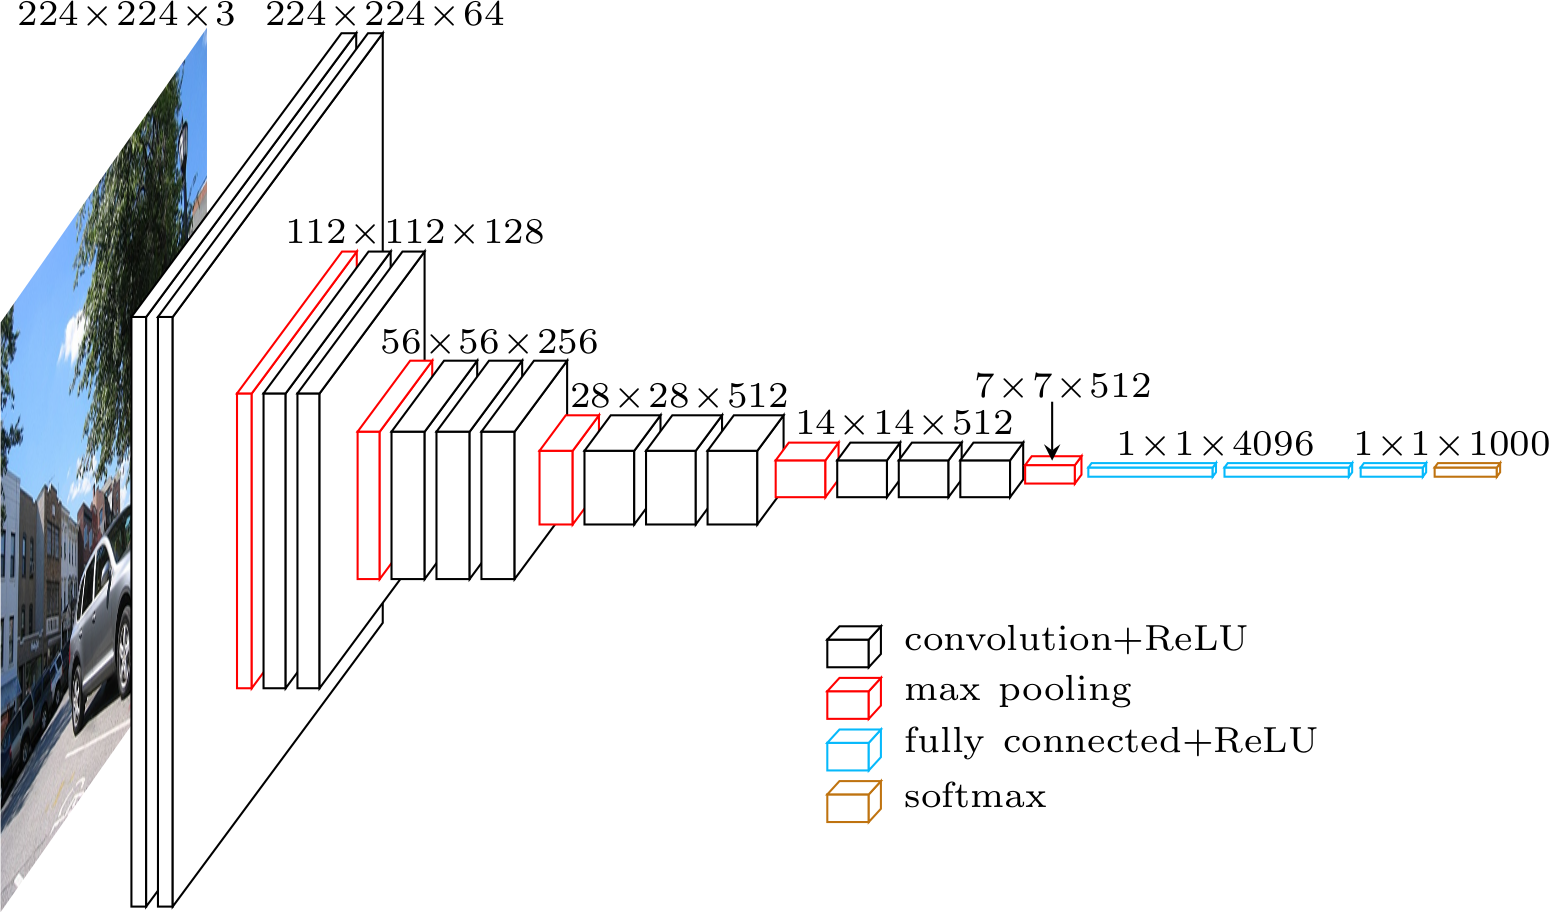
\includegraphics[width=9cm]{figure/alexnet.png}}%
\only<2>{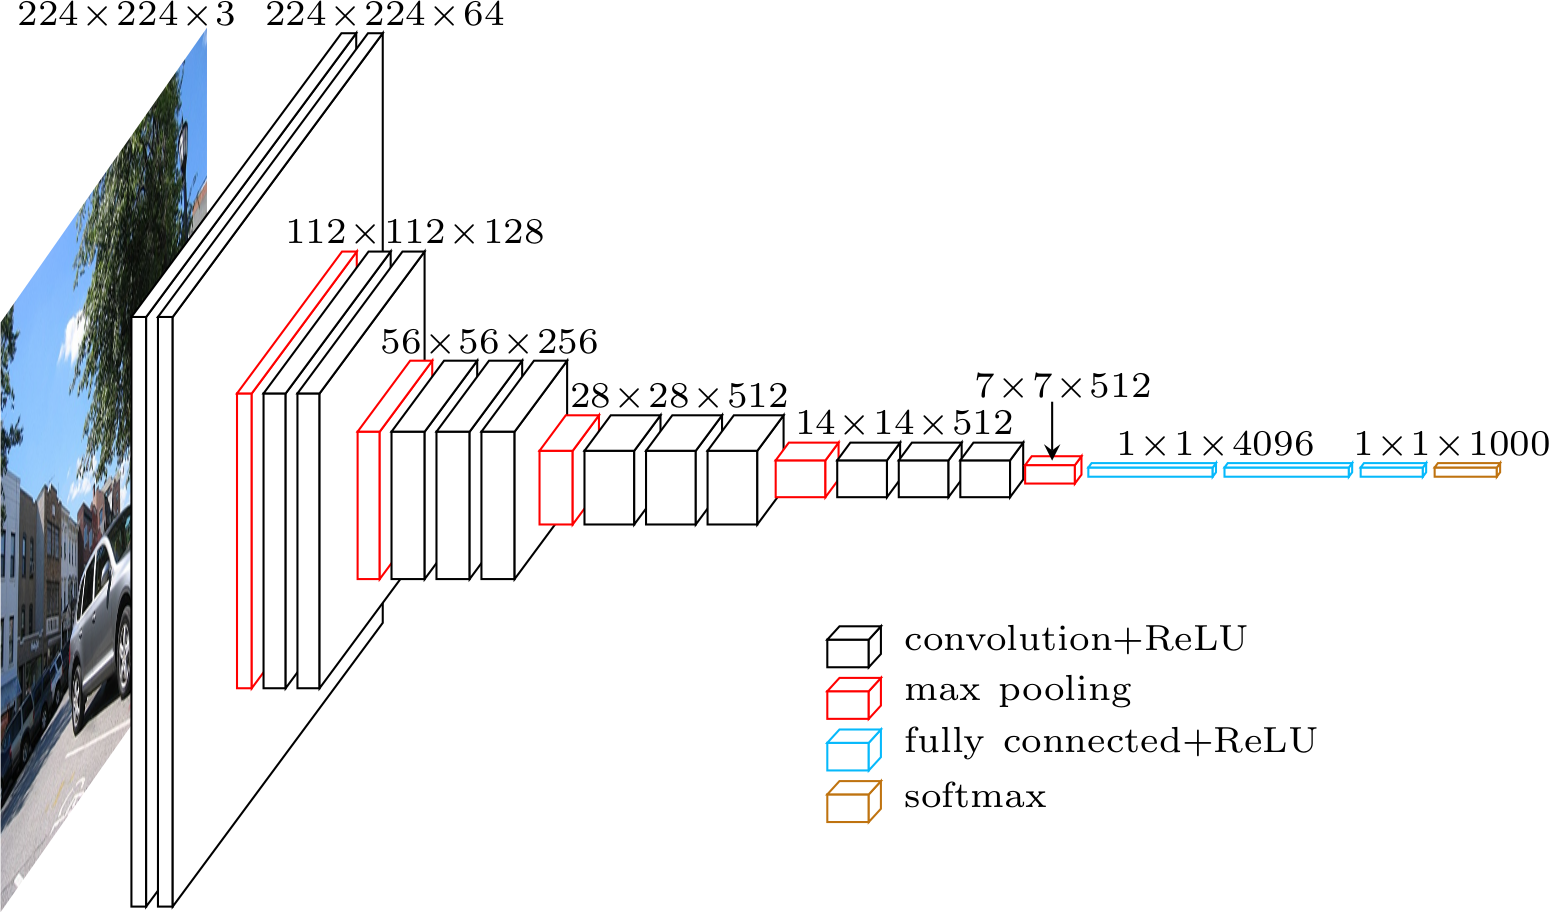
\includegraphics[width=9cm]{figure/alexnet.png}}%
\begin{itemize}
\only<1>{\item Input layer: contains the input (-image) as data matrices.}
\only<1>{\item \textbf{Convolutions}: extract feature maps from a previous layer.}
\only<1>{\item \textbf{Pooling}: reduces the dimensionality of any input and filter robust features.}
\only<2>{\item Fully connected layer: standard layer that connects feature map elements with the output neurons.}
\only<2>{\item Softmax: squashes output values to probability scores.}
\end{itemize}
\end{frame}
%%%%%%%%%%%%%%%%%%%%%%%%%%%%%%%%%%%%%%%%%%%%%%%%%%%%%%%%%%%%%%%%%%

\endlecture
\end{document}